\documentclass[conference]{IEEEtran}
% ---------------------------------------------------------------------------
% Before submission:
%  * replace the author block with the real names, department and e-mails;
%  * check the target conference's page limit and template version;
%  * IEEE requires disclosure of AI-generated content: keep or adapt the
%    acknowledgment sentence that discloses AI assistance.
% ---------------------------------------------------------------------------
\usepackage{cite}
\usepackage{amsmath,amssymb}
\usepackage{graphicx}
\usepackage{booktabs}
\usepackage{multirow}
\usepackage{tikz}
\usetikzlibrary{positioning,arrows.meta,calc,fit}
\usepackage[hidelinks]{hyperref}
\graphicspath{{../results/}}

\begin{document}

\title{A Significance-Driven Hybrid Approximate 8$\times$8 Multiplier for LUT-Constrained FPGAs in Error-Tolerant Image Processing}

\author{
\IEEEauthorblockN{Student Name 1, Student Name 2, Student Name 3}
\IEEEauthorblockA{\textit{Department of Electronics and Communication Engineering}\\
\textit{College Name}, City, India\\
student1@college.edu}
\and
\IEEEauthorblockN{Guide Name}
\IEEEauthorblockA{\textit{Department of Electronics and Communication Engineering}\\
\textit{College Name}, City, India\\
guide@college.edu}
}

\maketitle

\begin{abstract}
Multipliers dominate the logic cost of image-processing and machine-learning datapaths on FPGAs, yet many such workloads tolerate small arithmetic errors. This paper presents a family of recursive 8$\times$8 unsigned multipliers, built from 2$\times$2 blocks, in which approximation is applied selectively to the least-significant partial products. Five approximate configurations are compared against an exact reference: Kulkarni-style under-designed 2$\times$2 blocks applied at three significance levels, truncation of the lowest 4$\times$4 partial product, and a hybrid (HYB) that combines truncation of the lowest block with approximate middle blocks. All designs were verified exhaustively over the 65{,}536 input pairs and synthesised for the Xilinx 7-series (Artix-7) fabric. The hybrid design uses 80 LUTs instead of 112 (a 28.6\% reduction) with a normalised mean error distance of 0.24\%. In three image-processing applications driven by the RTL product tables, it keeps PSNR between 46.7 and 50.1\,dB and SSIM at or above 0.996. The exploration also shows that truncating the lowest partial product is Pareto-superior to applying the under-designed 2$\times$2 block in the upper partial products at the LUT granularity of the target fabric.
\end{abstract}

\begin{IEEEkeywords}
approximate computing, approximate multiplier, FPGA, Verilog, LUT optimisation, image processing
\end{IEEEkeywords}

% ===========================================================================
\section{Introduction}
Approximate computing trades a controlled loss of accuracy for savings in area, delay and energy in applications whose outputs are judged by humans or by statistical quality metrics~\cite{han2013approximate,mittal2016survey}. Multipliers are a natural target, because they are the most expensive arithmetic operator in filters, transforms and neural-network layers~\cite{jiang2020survey}.

Most approximate multipliers were designed for ASICs, where savings are counted in transistors or gates. On an FPGA the cost unit is different: logic is implemented in 6-input look-up tables (LUTs) and dedicated carry chains~\cite{ug474}. A simplification that removes a gate does not necessarily remove a LUT, which is why FPGA-specific approximate multipliers have been proposed~\cite{ullah2022fpga,vakili2024dyrecmul}. Even for exact arithmetic, a hand-structured 4-bit multiplier can use fewer LUTs than the netlist inferred from a behavioural \texttt{a*b}~\cite{kida2025fourbit}.

This paper asks a simple, practical question: \emph{where} in a recursive multiplier should approximation be placed to obtain the best LUT-versus-accuracy trade-off on a low-cost FPGA? The contributions are:
\begin{itemize}
\item A parameterised Verilog family of six 8$\times$8 multipliers (one exact, five approximate) built from 2$\times$2 blocks, with approximation placed by partial-product significance.
\item Exhaustive functional verification and error characterisation (error rate, MED, NMED, MRED, worst-case error) over all 65{,}536 input pairs.
\item A synthesis study for the Xilinx 7-series fabric used on the Basys-3 teaching board~\cite{basys3rm}, showing that a hybrid of truncation and approximation (HYB) saves 28.6\% of LUTs.
\item An application study (image multiplication, Gaussian smoothing and image blending) in which every multiplication is taken from the RTL simulation output.
\end{itemize}

% ===========================================================================
\section{Background and Related Work}
\subsection{Recursive multiplication}
An $n\times n$ product can be decomposed into four $n/2\times n/2$ partial products. With $A=\{A_H,A_L\}$ and $B=\{B_H,B_L\}$ split into 4-bit halves,
\begin{equation}
AB = 2^{8}A_HB_H + 2^{4}(A_HB_L + A_LB_H) + A_LB_L .
\label{eq:rec}
\end{equation}
Each 4$\times$4 term is decomposed again into 2$\times$2 terms with weights $2^4$, $2^2$ and $2^0$. The weights in~\eqref{eq:rec} show that an error in $A_LB_L$ is scaled by $2^0$, whereas an error in $A_HB_H$ is scaled by $2^8$.

\subsection{Under-designed 2$\times$2 multiplier}
Kulkarni \emph{et al.}~\cite{kulkarni2011udm} observed that an exact 2$\times$2 multiplier needs a fourth output bit only for $3\times3=9$. Their approximate block returns $7$ for that single input pair and is exact otherwise, so its output fits in three bits:
\begin{equation}
p_0 = a_0b_0,\quad p_1 = a_1b_0 \lor a_0b_1,\quad p_2 = a_1b_1 .
\end{equation}
One of the 16 input combinations is wrong, and the result always under-estimates the true product.

\subsection{FPGA-oriented approximate multipliers}
Architectural-space exploration of approximate multipliers~\cite{rehman2016space} and FPGA-specific designs that exploit LUT and carry-chain structure~\cite{ullah2022fpga} show that FPGA savings differ from ASIC savings. DyRecMul uses dynamically reconfigurable LUTs to cut LUT usage by 64\% for signed 8-bit multiplication on an UltraScale+ device~\cite{vakili2024dyrecmul}, and hand-optimised exact small multipliers can beat synthesis-inferred ones~\cite{kida2025fourbit}. This work is deliberately simpler: it uses only standard Verilog and a significance-driven placement rule, so the designs can be reproduced with open-source tools and a low-cost board.

% ===========================================================================
\section{Proposed Multiplier Family}
\begin{figure}[t]
\centering
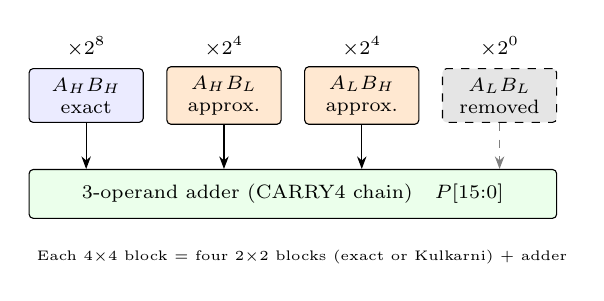
\begin{tikzpicture}[
  blk/.style={draw, rounded corners=1.5pt, minimum width=1.45cm, minimum height=0.62cm, font=\scriptsize, align=center},
  ex/.style={blk, fill=blue!8},
  ap/.style={blk, fill=orange!18},
  tr/.style={blk, fill=gray!20, dashed},
  >={Stealth[length=1.6mm]}]
\node[ex] (hh) at (0,0)      {$A_HB_H$\\exact};
\node[ap] (hl) at (1.75,0)   {$A_HB_L$\\approx.};
\node[ap] (lh) at (3.5,0)    {$A_LB_H$\\approx.};
\node[tr] (ll) at (5.25,0)   {$A_LB_L$\\removed};
\node[font=\scriptsize] at (0,0.62)    {$\times 2^{8}$};
\node[font=\scriptsize] at (1.75,0.62) {$\times 2^{4}$};
\node[font=\scriptsize] at (3.5,0.62)  {$\times 2^{4}$};
\node[font=\scriptsize] at (5.25,0.62) {$\times 2^{0}$};
\node[blk, minimum width=6.7cm, fill=green!8] (add) at (2.625,-1.25) {3-operand adder (CARRY4 chain)\quad $P[15{:}0]$};
\foreach \n in {hh,hl,lh} \draw[->] (\n.south) -- (\n.south |- add.north);
\draw[->, dashed, gray] (ll.south) -- (ll.south |- add.north);
\node[font=\tiny, align=left, anchor=west] at (-0.75,-2.05) {Each 4$\times$4 block = four 2$\times$2 blocks (exact or Kulkarni) + adder};
\end{tikzpicture}
\caption{Partial-product structure of the 8$\times$8 multiplier, shown for the proposed hybrid (HYB) configuration. Approximation is applied only to the lower-weight partial products.}
\label{fig:arch}
\end{figure}

\subsection{Design space}
Fig.~\ref{fig:arch} shows the partial-product structure. A single Verilog module, \texttt{mul8x8}, takes a \texttt{MODE} parameter that sets, for each 4$\times$4 partial product, whether it is exact, built from approximate 2$\times$2 blocks, or removed:
\begin{itemize}
\item \textbf{EXACT}: all blocks exact (reference).
\item \textbf{AM-L}: $A_LB_L$ approximate.
\item \textbf{AM-LM}: $A_LB_L$, $A_HB_L$ and $A_LB_H$ approximate.
\item \textbf{AM-ALL}: all four blocks approximate~\cite{kulkarni2011udm}.
\item \textbf{TRUNC-L}: $A_LB_L$ removed (forced to zero).
\item \textbf{HYB} (proposed): $A_LB_L$ removed and $A_HB_L$, $A_LB_H$ approximate; $A_HB_H$ exact.
\end{itemize}
The rule is significance-driven: approximation is added from the lowest weight upwards, and the most significant block $A_HB_H$ is kept exact in every design except AM-ALL. Because every variant only removes or under-estimates partial products, all approximate products satisfy $\tilde{P}\le AB$. This property was checked exhaustively, and it makes the error one-sided and easy to compensate if needed.

\subsection{Implementation}
The RTL uses three modules (\texttt{mul2x2}, \texttt{mul4x4}, \texttt{mul8x8}) with \texttt{generate} blocks selecting exact or approximate sub-blocks. A registered wrapper (\texttt{mul8x8\_pipe}) places the multiplier between input and output registers for clocked use. A Basys-3 top level instantiates all six multipliers: switches provide the operands, LEDs show the product, push-buttons select the mode, and the seven-segment display shows the mode and the error magnitude $|AB-\tilde{P}|$.

% ===========================================================================
\section{Evaluation Methodology}
\textbf{Functional verification.} A self-checking Icarus Verilog~\cite{iverilog} testbench applies all $256\times256$ input pairs to every design. It checks that the exact recursive design and the behavioural \texttt{a*b} both equal the reference product, and that no approximate design over-estimates it. All 65{,}536 products of every design are written to a file. An independent Python model of each design reproduces the RTL output bit for bit.

\textbf{Error metrics.} With error distance $ED = |AB-\tilde{P}|$ and $P_{\max}=255^2$, we report the error rate (ER, fraction of inputs with $ED>0$), mean error distance (MED), normalised MED (NMED $=$ MED$/P_{\max}$), mean relative error distance (MRED, over non-zero products) and worst-case error (WCE)~\cite{jiang2020survey}.

\textbf{Synthesis.} Designs were synthesised with Yosys~\cite{yosys} (\texttt{synth\_xilinx -family xc7 -nodsp}) for the 7-series fabric of the Artix-7 XC7A35T on the Basys-3 board~\cite{basys3rm}. DSP inference was disabled so that all designs are compared in LUTs and CARRY4 cells~\cite{ug474}. The primary flow preserves hierarchy, so each block is mapped as designed. A fully flattened ABC9 flow is reported as a sensitivity check. Logic depth is the longest path in mapped cells, excluding I/O buffers.

\textbf{Applications.} Three 8-bit kernels were run on standard $512\times512$ greyscale test images from scikit-image~\cite{vanderwalt2014skimage}, using only the RTL product tables: (i) pixel-wise image multiplication, $(I_1I_2)\gg8$; (ii) 3$\times$3 Gaussian smoothing with integer weights $\{20,32,48\}$ summing to 256~\cite{gonzalez2018dip}; and (iii) alpha blending with $\alpha=179/255$. Quality is measured against the exact output with PSNR and SSIM~\cite{wang2004ssim}.

% ===========================================================================
\section{Results}
\subsection{Functional verification and waveforms}
The exhaustive testbench reported zero mismatches for the exact designs and zero over-estimations for the approximate designs. Fig.~\ref{fig:wave} shows the clocked simulation at 100\,MHz. Products appear two cycles after their operands. The $3\times3$ case returns 7 in the three AM designs. TRUNC-L and HYB return 0 for any pair whose upper nibbles are both zero (e.g.\ $12\times10$, $3\times3$, $15\times15$), because the whole product then lies in the removed $A_LB_L$ term. The $255\times255$ case shows the error growing with the number of approximated blocks.

\begin{figure*}[t]
\centering
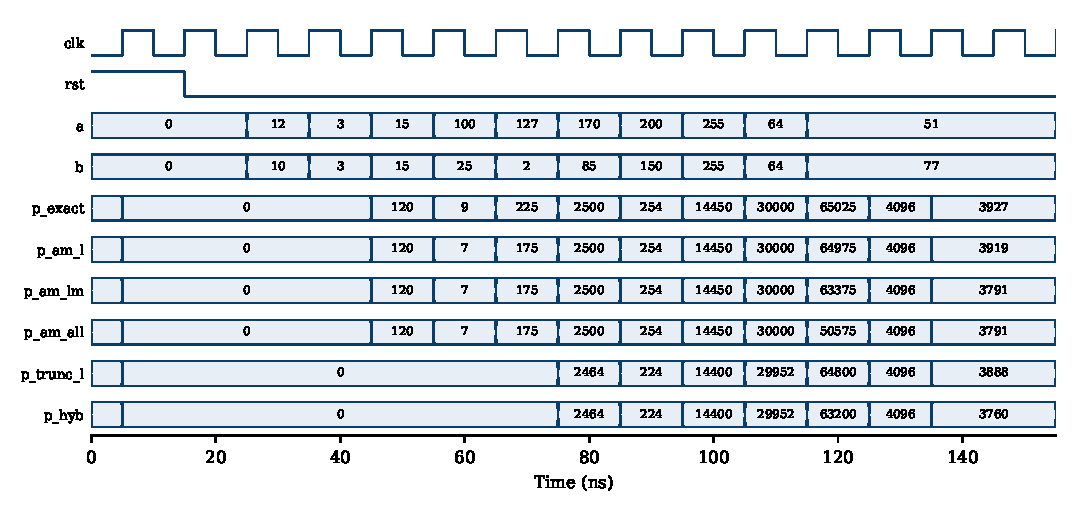
\includegraphics[width=0.92\textwidth]{fig_waveform.pdf}
\caption{Simulation waveform (Icarus Verilog, 100\,MHz clock). Products appear two cycles after the operands. For $a=b=255$ the outputs are 65025 (EXACT), 64975 (AM-L), 63375 (AM-LM), 50575 (AM-ALL), 64800 (TRUNC-L) and 63200 (HYB).}
\label{fig:wave}
\end{figure*}

\subsection{Error characteristics}
Table~\ref{tab:err} lists the error metrics. Approximating only $A_LB_L$ (AM-L) produces a very small NMED of 0.0048\%, while applying the under-designed block everywhere (AM-ALL) raises the worst-case error to 22.2\% of full scale. TRUNC-L has a high error rate (87.9\%) but a bounded worst-case error of 225, because the removed partial product is at most $15\times15$. HYB inherits that bound for its lowest block and adds the small middle-block error, reaching NMED~0.24\%.

\begin{table}[t]
\centering
\caption{Error metrics over all 65{,}536 input pairs}
\label{tab:err}
\setlength{\tabcolsep}{4pt}
\begin{tabular}{lrrrrr}
\toprule
Design & ER (\%) & MED & NMED (\%) & MRED (\%) & WCE \\
\midrule
EXACT   & 0.00  & 0.00   & 0.0000 & 0.000 & 0 \\
AM-L    & 19.14 & 3.12   & 0.0048 & 0.076 & 50 \\
AM-LM   & 40.67 & 103.12 & 0.1586 & 0.925 & 1650 \\
AM-ALL  & 46.73 & 903.12 & 1.3889 & 3.280 & 14450 \\
TRUNC-L & 87.89 & 56.25  & 0.0865 & 1.859 & 225 \\
\textbf{HYB} & 90.28 & 156.25 & 0.2403 & 2.708 & 1825 \\
\bottomrule
\end{tabular}
\end{table}

\begin{figure*}[t]
\centering
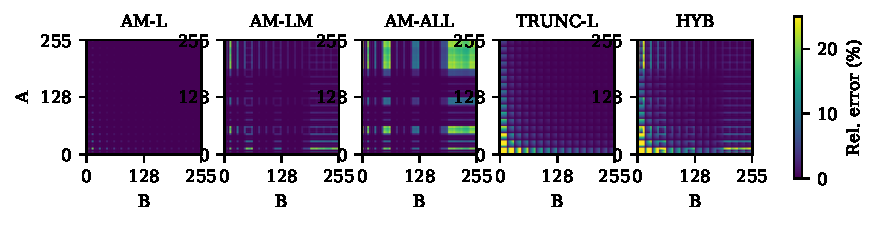
\includegraphics[width=0.95\textwidth]{fig_error_map.pdf}
\caption{Relative error over the operand space ($A$ vertical, $B$ horizontal; colour scale clipped at 25\%). For TRUNC-L and HYB the largest relative errors occur at small operands, where the removed $A_LB_L$ term is a large fraction of the product. AM-ALL also errs at large operands, because its most significant block $A_HB_H$ is approximated.}
\label{fig:map}
\end{figure*}

\subsection{FPGA resources}
Table~\ref{tab:syn} gives the synthesis results. In the hierarchy-preserving flow, the exact recursive design uses 112 LUTs, practically the same as the behavioural \texttt{a*b} (113 LUTs plus 23 wide-mux cells). Each approximate 2$\times$2 block saves one LUT because its fourth output is constant, so AM-L, AM-LM and AM-ALL save 4, 12 and 16 LUTs. Removing $A_LB_L$ saves a whole 4$\times$4 block and two CARRY4 cells, and shortens the longest path by one cell. HYB combines both effects: 80 LUTs, a 28.6\% reduction.

\begin{table}[t]
\centering
\caption{Synthesis results, Xilinx 7-series (Yosys, no DSP)}
\label{tab:syn}
\setlength{\tabcolsep}{3.4pt}
\begin{tabular}{lrrrrr}
\toprule
 & \multicolumn{4}{c}{Hierarchical (primary)} & Flat \\
\cmidrule(lr){2-5}
Design & LUT & CARRY4 & Depth & Saving & LUT \\
\midrule
Behavioural \texttt{a*b} & 113$^\dagger$ & 4 & 9 & $-0.9$\% & 103 \\
EXACT   & 112 & 12 & 8 & -- & 103 \\
AM-L    & 108 & 12 & 8 & 3.6\% & 120 \\
AM-LM   & 100 & 12 & 8 & 10.7\% & 97 \\
AM-ALL  & 96  & 12 & 8 & 14.3\% & 88 \\
TRUNC-L & 88  & 10 & 7 & 21.4\% & 82 \\
\textbf{HYB} & \textbf{80} & 10 & 7 & \textbf{28.6\%} & \textbf{62} \\
\bottomrule
\multicolumn{6}{l}{\footnotesize $^\dagger$plus 22 MUXF7 and 1 MUXF8; with DSP inference: 1 DSP48E1.}
\end{tabular}
\end{table}

The flattened ABC9 flow lets the tool re-optimise across block boundaries. It confirms the ordering for the most aggressive designs (HYB: 62 LUTs versus 103 for EXACT, a 39.8\% reduction), but it is not monotonic for the lightest approximation: AM-L grows to 120 LUTs. Savings from small approximations are therefore sensitive to synthesis heuristics, whereas the structural savings of truncation and HYB hold in both flows.

\subsection{Accuracy--area trade-off}
Fig.~\ref{fig:trade} plots LUTs against NMED. TRUNC-L is both smaller and more accurate than AM-LM and AM-ALL, so applying the under-designed block to the middle and upper partial products is dominated by simply removing the lowest one. The Pareto front is formed by EXACT, AM-L, TRUNC-L and HYB. HYB gives the lowest LUT count for NMED below 0.25\%.

\begin{figure}[t]
\centering
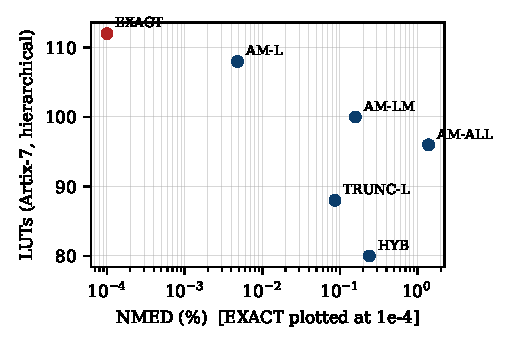
\includegraphics[width=\columnwidth]{fig_tradeoff.pdf}
\caption{LUT count versus NMED. EXACT is plotted at $10^{-4}$ for the log axis. EXACT, AM-L, TRUNC-L and HYB form the Pareto front.}
\label{fig:trade}
\end{figure}

\subsection{Image-processing quality}
Table~\ref{tab:img} and Fig.~\ref{fig:img} report the application results. All designs except AM-ALL keep PSNR above 46\,dB and SSIM of at least 0.996, a level at which differences are not visible. AM-L is bit-identical to EXACT in Gaussian smoothing, because an AM-L error needs a 2-bit field equal to 3 in the low nibble of both operands, and the low nibbles of the kernel weights (20, 32, 48) never contain one. AM-ALL drops to about 34--35\,dB, which is consistent with its much larger worst-case error.

\begin{table}[t]
\centering
\caption{Image quality versus exact output: PSNR (dB) / SSIM}
\label{tab:img}
\setlength{\tabcolsep}{3pt}
\begin{tabular}{lccc}
\toprule
Design & Multiplication & Gaussian & Blending \\
\midrule
AM-L    & 64.81 / 0.9998 & identical      & 60.93 / 0.9996 \\
AM-LM   & 51.99 / 0.9973 & 56.17 / 0.9988 & 49.38 / 0.9980 \\
AM-ALL  & 35.27 / 0.9851 & 34.98 / 0.9959 & 34.16 / 0.9951 \\
TRUNC-L & 55.70 / 0.9984 & 51.50 / 0.9976 & 51.99 / 0.9980 \\
\textbf{HYB} & 50.12 / 0.9960 & 49.71 / 0.9972 & 46.66 / 0.9975 \\
\bottomrule
\end{tabular}
\end{table}

\begin{figure*}[t]
\centering
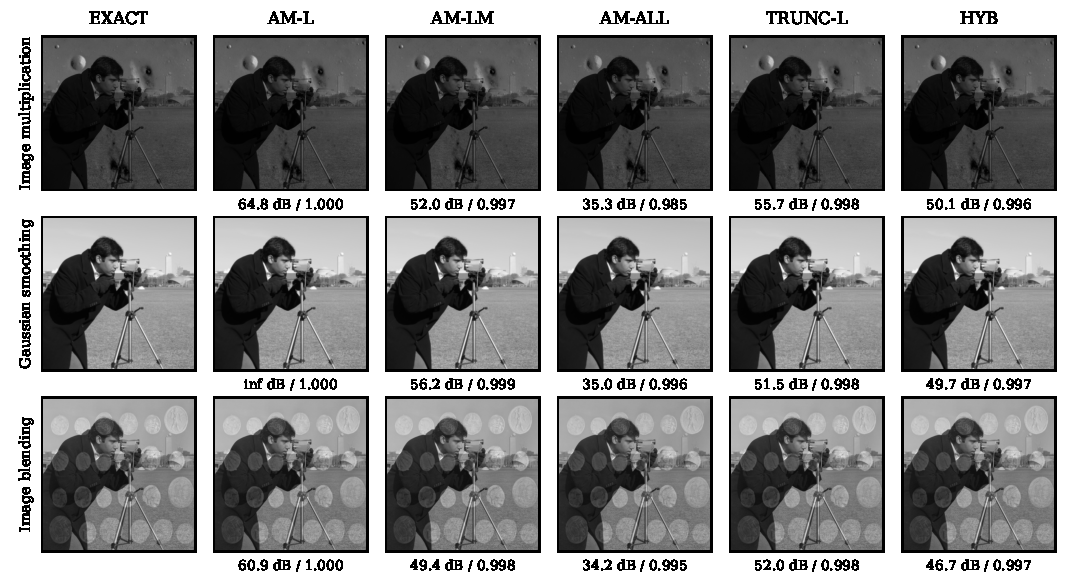
\includegraphics[width=0.9\textwidth]{fig_images.pdf}
\caption{Outputs of the three image kernels computed with the RTL product tables of each multiplier. Labels give PSNR / SSIM against the exact output.}
\label{fig:img}
\end{figure*}

\subsection{Discussion and limitations}
The results support a simple design rule for LUT-based FPGAs: remove the lowest-weight partial product first, and approximate the middle ones only if more area must be saved. Two limitations should be noted. First, resources were obtained with an open-source synthesis flow. Vendor place-and-route (Vivado) timing and power figures for the Basys-3 board are needed to quantify delay and energy, and absolute LUT counts will differ from Vivado's. Second, TRUNC-L and HYB return zero when both operands are below 16, so they suit data dominated by mid-to-high values (such as natural images) but not kernels that multiply many small numbers. Their error is also one-sided (biased low), and a constant compensation term could reduce MED further at negligible cost.

% ===========================================================================
\section{Conclusion}
A parameterised family of recursive 8$\times$8 approximate multipliers was designed in Verilog, verified exhaustively, synthesised for the Xilinx 7-series fabric and evaluated in three image-processing kernels. Significance-driven placement matters: removing the least-significant 4$\times$4 partial product beats applying the under-designed 2$\times$2 block in higher partial products. Combining the two in the proposed HYB design saves 28.6\% of LUTs (39.8\% in a flattened flow) with NMED 0.24\% and image PSNR of at least 46.7\,dB. Future work includes Vivado implementation with timing and power measurement on the Basys-3 board, bias compensation, and integration into a convolution accelerator.

\section*{Acknowledgment}
The authors thank the Department of Electronics and Communication Engineering, College Name, for laboratory support. Parts of this manuscript and its Verilog code were drafted with the assistance of an AI tool; the authors reviewed, verified and take responsibility for all content.

\bibliographystyle{IEEEtran}
\bibliography{refs}

\end{document}
